\chapter{Safety and assurance}

In \cite{Amodei}, five major research problems associated with unsafe behaviour of ML models is presented. They can be summarized as
\begin{enumerate}
	\item Avoiding Negative Side Effects: How to ensure that the model will not disturb the environment while pursuing its goals, e.g. can a cleaning robot knock over a vase because it can clean faster by doing so? Can we do this without manually specifying everything the robot should not disturb \cite{Amodei}?
	
	\item Avoiding Reward Hacking: How to ensure that the model does not avoid situations to achieve a higher reward. For example, if we reward the robot for achieving an environment free of messes, it might disable its vision so that it won’t find any messes, or cover over messes with materials it can’t see through, or simply hide when humans are around so they can’t tell it about new types of messes \cite{Amodei}. 
	
	\item Scalable Oversight: How to ensure the model respects the parts of the objective function that are expensive to evaluate and makes a safe approximation of these parts. 
	For example, in the cleaning robot example, if the user is happy with the cleaning quality is an expensive objective function, but it can be approximated to presence of any dirt on the floor when the user arrives \cite{Amodei}. 
	
	\item Safe Exploration: How to ensure that the ML model explorations are safe. For example, the robot should experiment with mopping strategies, but putting a wet mop in an electrical outlet is a very bad idea \cite{Amodei}. 
	
	\item Robustness to Distributional Shift: How to ensure that the model performs robustly if the environment shifts from the training environment. For example, strategies a cleaning robot learns for cleaning an office might be dangerous on a factory workfloor \cite{Amodei}.

\end{enumerate}
% This is a sample chapter

% \section{Referencing}
% % These are some sample references to GAMYGDALA~\citep{popescu2014gamygdala} from the ``refernces.bib" file and state effects of cognition~\citep{hudlicka2002time} from the ``reference\_another.bib" file. These references are not in the same .bib file.

% \section{Figures}
% This is a single image figure (Figure~\ref{fig_singleenv}:

% \begin{figure}[ht]
% 	\centering
% 	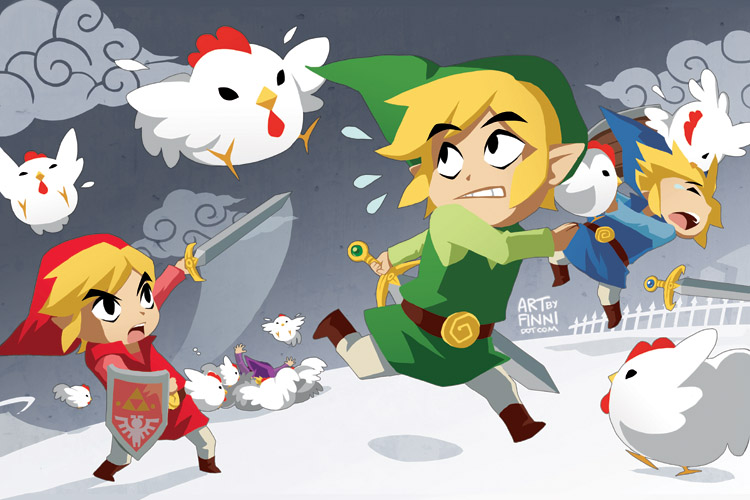
\includegraphics[width=0.6\textwidth]{figures/Sample/tumblr_static_eaceks0rfxsss8o4swscw40wo.jpg}
% 	\caption[Single Figure Environment Listed Title]{This is a single figure environment}
% 	\label{fig_singleenv}
% \end{figure}

% This is a multi-image figure with a top (Figure~\ref{fig_multienv_1}) and bottom (Figure~\ref{fig_multienv_2}) aligned subfigures:

% \begin{figure}[ht]
% 	\centering
% 	\begin{subfigure}[t]{\textwidth}
% 		\centering
% 		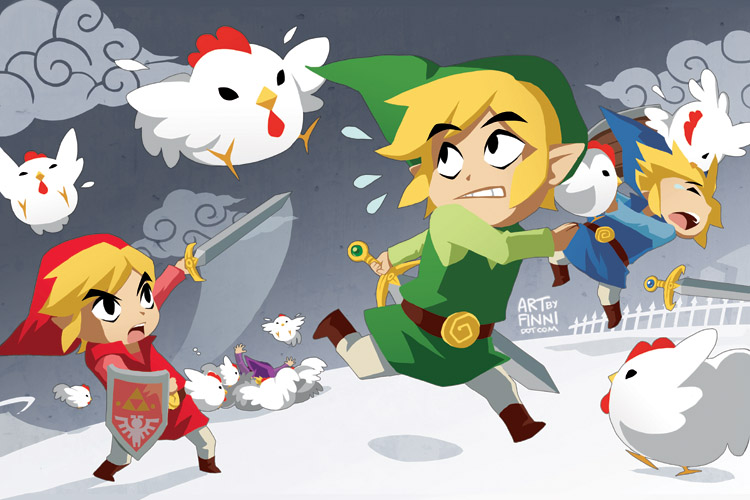
\includegraphics[width=0.7\textwidth]{figures/Sample/tumblr_static_eaceks0rfxsss8o4swscw40wo.jpg}
% 		\caption{Figure 1}
% 		\label{fig_multienv_1}
% 	\end{subfigure}
% 	~
% 	\begin{subfigure}[t]{\textwidth}
% 		\centering
% 		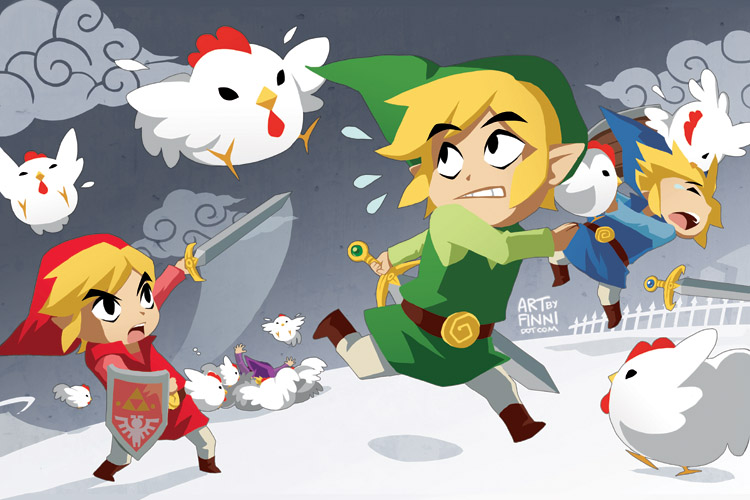
\includegraphics[width=0.7\textwidth]{figures/Sample/tumblr_static_eaceks0rfxsss8o4swscw40wo.jpg}
% 		\caption{Figure 2}
% 		\label{fig_multienv_2}
% 	\end{subfigure}
	
% 	\caption{A Multi-Figure Environment}
% 	\label{fig_multienv}
% \end{figure}

% \section{Tables}

% Here is a sample table (Table~\ref{tab_sample}):

% 	\begin{table}[ht]
% 	\centering
% 	\begin{tabular}{ m{0.2\textwidth} m {0.1\textwidth} m{0.15\textwidth} }
% 		\toprule
% 		A & $\longleftrightarrow$ & B \\
% 		C & $\longleftrightarrow$ & D \\
% 		\bottomrule	
% 	\end{tabular}	
% 	\caption{A sample table}	
% 	\label{tab_sample}
% \end{table}

% \subsection{Long Tables}
% A sample long table is shown in Appendix~\ref{appendix_b}.

% \section{Equations}

% Here is a sample equation (Equation~\ref{eq_lineslope}):

% \begin{equation} \label{eq_lineslope}
% 	y = mx + b
% \end{equation}